\documentclass[12pt,twocolumn]{article} 
\usepackage{geometry}
 \geometry{
  a4paper,
  left=17.5mm,
  right=17.5mm,
  bottom=15mm,
  top=15mm
 }
\usepackage[english]{babel}
\usepackage{subcaption}
\usepackage{tikz}
\usetikzlibrary{decorations.pathreplacing}
\usepackage{textcomp}
\usepackage{float}
\usepackage{amsmath}
\tikzset{XOR/.style={draw,circle,append after command={
        [shorten >=\pgflinewidth, shorten <=\pgflinewidth,]
        (\tikzlastnode.north) edge (\tikzlastnode.south)
        (\tikzlastnode.east) edge (\tikzlastnode.west)
        }
    }
}
\usepackage{graphicx,booktabs,array}

\title{\bf \Huge A practical application of EOS\textregistered{} projection geometry}
\author{{\bf \Large Anthony J. Lombard$^{1,2}$}\\
  $^1$ Medical Computing Team, Kitware Inc.,\\
  Albany, NY, USA\\
  $^2$ Department of Computer Science, Clarkson University,\\ 
  Potsdam, NY, USA
  }
\date{April 26th 2024}

\begin{document}
\maketitle

Accurately rendering 3D volumes into synthetic radiographs or digitally reconstructed radiographs (DRRs) 
is an important step in many biomedical research applications. While many techniques, such as ray-casting, have been 
established in this field, they rely on the traditional pinhole camera model. While this model is quite accurate for 
most applications, when complex and strange geometry is required, such as the EOS\textregistered{} radiographic 
scanner, this simple camera model can break down and produce results that are not accurate. In this paper I will show 
a modified pinhole camera model for ray-casting to more accurately describe the geometry of the EOS\textregistered{} 
system.
\noindent
{\bf Keywords:} Ray-casting, Synthetic Radiographs, DRR, Autoscoper, EOS\textregistered{}

\section{Introduction}

The EOS\textregistered{} radiographic scanner is unique system that allows for full-body radiography. 
The ability to be able to quickly render Digitally Reconstructed Radiographs (DRRs) is a necessary step to perform
many different forms of analysis later on, such as 2D-3D registration. 

While previous publications have defined volume-order rendering techniques for this scanner \cite{groisser2019geometry},
there has not been any development towards image-order rendering. Image-order techniques have a few advantages over 
volume-order techniques. Mainly, it is easier to parallelize image-order techniques for faster computation. It is also 
easier to render regions of interest (ROI) rather than the entire image.

This paper provides a detailed overview of DRR rendering using ray-casting, an overview of the EOS\textregistered{} 
geometry, and the modified ray-casting approach used to simulate the EOS\textregistered{} scanner.

\section{Ray-casting / DRR generation}
The basic idea of ray-casting is sending rays from a point source through a 3D scene to determine the value at each 
pixel in the final image. 

Let our camera be a static point in world space, C. 
Let the current pixel in the image be some point on the image plane in world space, I. 
Then the direction of travel for our ray would be the normalized result of I-C, we will call this R.

We can express a point, P, along this ray using the parametric form. Where t is the distance traveled along the ray.
\begin{equation}
  P = C + t * R
\end{equation}


\begin{equation}
  \text{pixel intensity} = \sum_{t=0,step\_size}^{dist(I,C)} value(C+t*R)
\end{equation}

In a naive approach, we could now get the intensity of each pixel using equation (2).
Where the function $dist$ returns the distance between two points, in this case the camera, C, and the pixel position I.
And the function $value$ returns the value of the volume at a given point, if the point lies outside of the volume it 
returns 0.
The $step\_size$ is the amount that t increments each iteration of the summation.

However, this approach has two major problems. 
First, it is likely that the volume does not take up the entire space between 
points C and I, so there would be many needless steps along the ray. We can solve this by using ray box intersection
to determine the values of t, if any, that the volumes resides in. Second, since the voxels of the volume are not 
clustered directly next to each other, there is some physical distance between points within the volume, it is likely 
that the point P won't fall directly on the center of a voxel. In the naive approach, we could simply take the value 
from the closest voxel. A better approach is to take the weighted average of the eight closest voxels, this is 
trilinear-interpolation \cite{Yoder_2003}.

\subsection{Ray box intersection}
In order to reduce the number of iterations needed to traverse each ray, ray-box intersection was utilized to 
determine the values for t that the volume fits between. We define the box based on the position and size of the volume
for all three axes. In total six planes are computed, in general this can be represented by the near and far planes
for each axis.
\begin{equation}
  box_{near} = \{X_{near}, Y_{near}, Z_{near}\}
\end{equation}
\begin{equation}
  box_{far} = \{X_{far}, Y_{far}, Z_{far}\}
\end{equation}
For each axis, the minimum and maximum extents for the box had the corresponding axial component 
of the ray origin subtracted from the extent, then the result of the subtraction is divided by the axial component 
of the ray direction. For example using the X-axis.
\begin{gather*}
  t_{xn} = (X_{near} - ray\_origin.x) / ray\_direction.x\\
  t_{xf} = (X_{far} - ray\_origin.x) / ray\_direction.x
\end{gather*}

We then find the minimum and maximum values for each axis and organize the results into two arrays, $tMin$ and $tMax$.
Where $tMin.x = min(t_{xn},t_{xf})$. Then the value for the near plane s computed as the maximum of the
$tMin$ array. Likewise the value for the far plane is computed as the minimum of the $tMax$ array.

If the value of the near plane is greater than that of the far plane, the ray missed the box. In which case we can end
computation early, saving more time and resources. 
\cite{glassnerIntro}

\section{Overview of the EOS\textregistered{} geometry}

The EOS\textregistered{} radiographic scanner contains two X-ray sources, that are mounted orthgonally from one
another. The two sources are physically linked so the two radiographic images are collected in unison. During a 
scan the sources are moved vertically.

\begin{figure}[H]
  \centering
  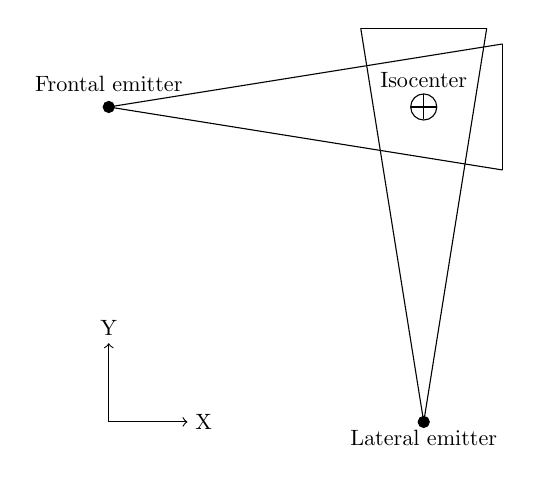
\begin{tikzpicture}
    % Frontal emitter
    \draw (0,0) -- (5,.8);
    \draw (0,0) -- (5,-.8);
    \draw (5,.8) -- (5,-.8);
    \filldraw (0,0) circle (2pt) node[above,scale=0.8] at (0,0.1) {Frontal emitter};

    % Lateral emitter
    \draw (4,-4) -- (3.2,1);
    \draw (4,-4) -- (4.8,1);
    \draw (3.2,1) -- (4.8,1);
    \filldraw (4,-4) circle (2pt) node[below, scale=0.8] {Lateral emitter};

    % Isocenter
    \draw (4,0) node[XOR]{} node[above,scale=0.8] at (4, 0.15) {Isocenter};

    % Axis
    \draw[->] (0,-4) -- (0,-3) node[above,scale=0.8] {Y};
    \draw[->] (0,-4) -- (1,-4) node[right,scale=0.8] {X};
  \end{tikzpicture}

  \caption{Top-down view of the EOS\textregistered{} geometry}
\end{figure}

Each source is at a known fixed position relative to each sources respective detector and the isocenter. 

\begin{figure}[H]
  \centering
  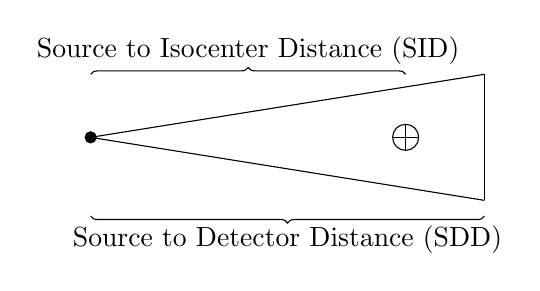
\begin{tikzpicture}
    \path[draw,decorate,decoration={brace}] (0,.8) -- (4,.8) node[midway,above]{Source to Isocenter Distance (SID)};
    % Frontal emitter
    \draw (0,0) -- (5,.8);
    \draw (0,0) -- (5,-.8);
    \draw (5,.8) -- (5,-.8);
    \filldraw (0,0) circle (2pt) node[above,scale=0.8] at (0,0.1) {};

    % Isocenter
    \draw (4,0) node[XOR]{} node[above,scale=0.8] at (4, 0.15) {};

    \path[draw,decorate,decoration={brace,mirror}] (0,-1) -- (5,-1) node[midway,below]{Source to Detector Distance (SDD)};
  \end{tikzpicture}
  \caption{Known fixed distances}
\end{figure}

Each radiograph image collected by the system can be of arbitrary size defined by the number of rows, R,
and the number of columns, C. The spacing between pixel centers is also known, the horizontal spacing is defined as
$\lambda$ and the vertical spacing is defined as $\lambda_z$.

\begin{figure}[H]
  \centering
  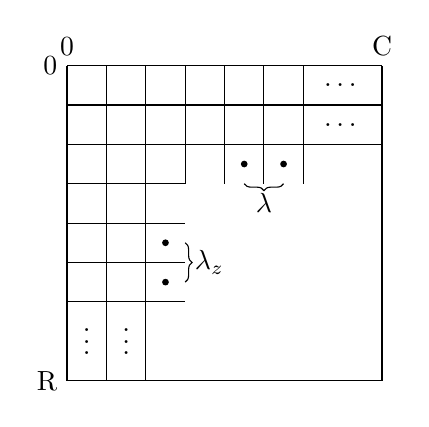
\begin{tikzpicture}[scale=2]
    \draw (0,0) node[above]{0} -- (2,0) node[above]{C};
    \draw (0,0) node[left] {0} -- (0,-2) node[left] {R};
    \draw (0,-2) -- (2,-2);
    \draw (2,-2) -- (2,0);

    % Horizontal Lines
    \draw (0,-0.25) -- (2,-.25);
    \draw (0,-0.5) -- (2,-.5);
    \draw (0,-0.75) -- (.75,-.75);
    \draw (0,-1) -- (.75,-1);
    \filldraw (0.625,-1.125) circle (0.5pt);
    \draw (0,-1.25) -- (.75,-1.25);
    \filldraw (0.625,-1.375) circle (0.5pt);
    \draw (0,-1.5) -- (.75,-1.5);

    \node[] at (1.75,-.125) {\dots};
    \node[] at (1.75,-.375) {\dots};
    
    \path[draw,decorate,decoration={brace}] (0.75 ,-1.125) -- (0.75,-1.375) node[midway,right]{$\lambda_z$};

    % Vertical Lines
    \draw (.25,0) -- (.25,-2);
    \draw (.5,0) -- (.5,-2);
    \draw (.75,0) -- (.75,-.75);
    \draw (1,0) -- (1,-.75);
    \filldraw (1.125,-.625) circle (0.5pt);
    \draw (1.25,0) -- (1.25,-.75);
    \filldraw (1.375,-.625) circle (0.5pt);
    \draw (1.5,0) -- (1.5,-.75);

    \node[] at (.125,-1.70) {\vdots};
    \node[] at (.375,-1.70) {\vdots};

    \path[draw,decorate,decoration={brace,mirror}] (1.125 ,-0.75) -- (1.375,-0.75) node[midway,below]{$\lambda$};
  \end{tikzpicture}
  \caption{Radiograph size and spacing}
\end{figure}


\section{EOS\textregistered{} geometry for DRR generation}

Note the subscript $f$ denotes a parameter specific to the frontal source. 
Likewise the subscript $l$ denotes a parameter specific to the lateral source.

Let v be the current vertical index in the DRR, where $v \in [0,R)$.

Let u be the current horizontal index in the DRR, where $u \in [0,C)$.

Let $z_0$ be the initial height of the scanner, then the current height of the scanner can then be defined as the 
current vertical index scaled by the vertical pixel spacing, then offset from the initial scanner height.

\begin{equation}
  z = z_0 - \lambda_z * v
\end{equation}

Defining the isocenter to be the point (0, 0, z) we can get the following positions, in world space, for the frontal 
and lateral sources.

\begin{equation}
  s_f = \{-sid_f,0,z\}
\end{equation}

\begin{equation}
  s_l = \{0,-sid_l,z\}
\end{equation}

The distance between the isocenter and each detector can be defined as the difference between each sources sdd and sid.
The position along each detector can be defined as the current horizontal index off set by half of the total number 
of columns in the image. This value then gets scaled by the horizontal pixel spacing and then divided by the focal
length. The ratio of sid to sdd is used as the focal length.

Therefore the current position on the detector, in world space, can be defined by the following equations.
\begin{equation}
  d_f = \{sdd_f-sid_f, \frac{(u - \frac{C_f}{2}) \cdot \lambda_f \cdot sdd_f}{sid_f},z\}
\end{equation}

\begin{equation}
  d_l = \{\frac{(u - \frac{C_l}{2}) \cdot \lambda_l \cdot sdd_l}{sid_l}, sdd_l-sid_l, z\}
\end{equation}

The ray-casting algorithm described in section 2, was then modified so the camera position was defined by $s$. The ray direction was then defined as the normalized result of $d-s$ the rest of the
algorithm was left as is.

\section{Results}

\subsection{Models in 3D}

Several models were kindly provided by Brown University \cite{AKHBARI2019120} for testing purposes.

\begin{figure}[H]
    \centering
    \begin{subfigure}[t]{0.25\textwidth}
        \centering
        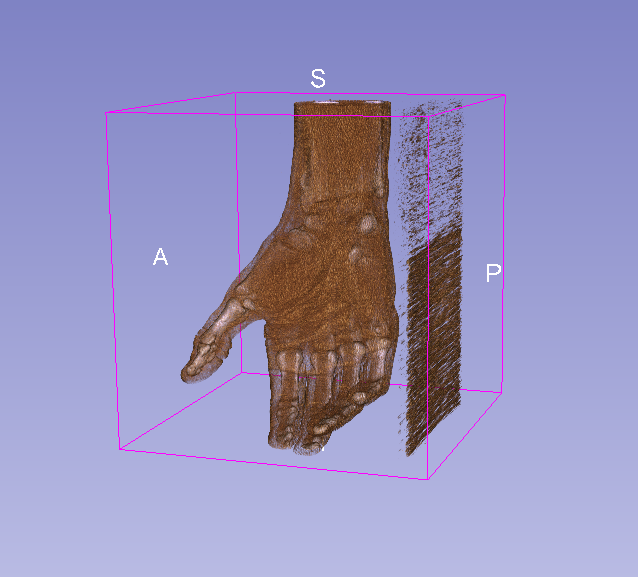
\includegraphics[height=1in]{img/hand-3d.png}
        \caption{Hand model}
    \end{subfigure}%
    ~ 
    \begin{subfigure}[t]{0.25\textwidth}
        \centering
        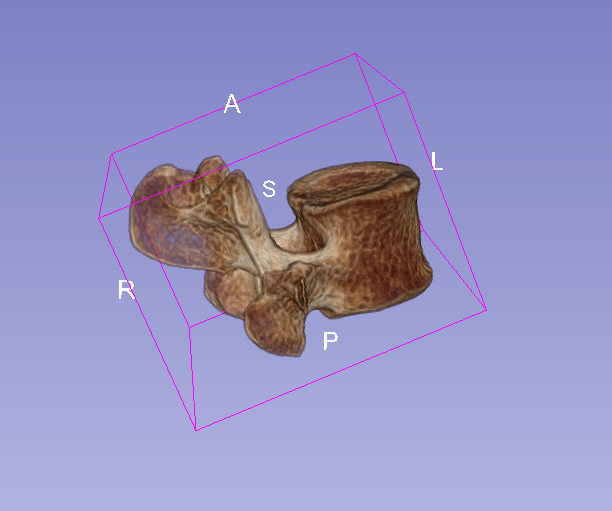
\includegraphics[height=1in]{img/vert-3d.png}
        \caption{Vertebrate model}
    \end{subfigure}
    \caption{Provided Models}
\end{figure}

\subsection{Projected Models}

Both of the models shown above were projected using the geometry described above. Parameters used to perform the
projections were those described by Groisser \cite{groisser2019geometry} about the EOS\textregistered{} installed 
in the Pediatric Radiology department at the Hospital for Special Surgery.

An image for each X-Ray source, frontal and lateral. The volume was also rotated 90$^{\circ}$ 
on each axis independently.

\begin{figure}[H]
  \begin{center}
    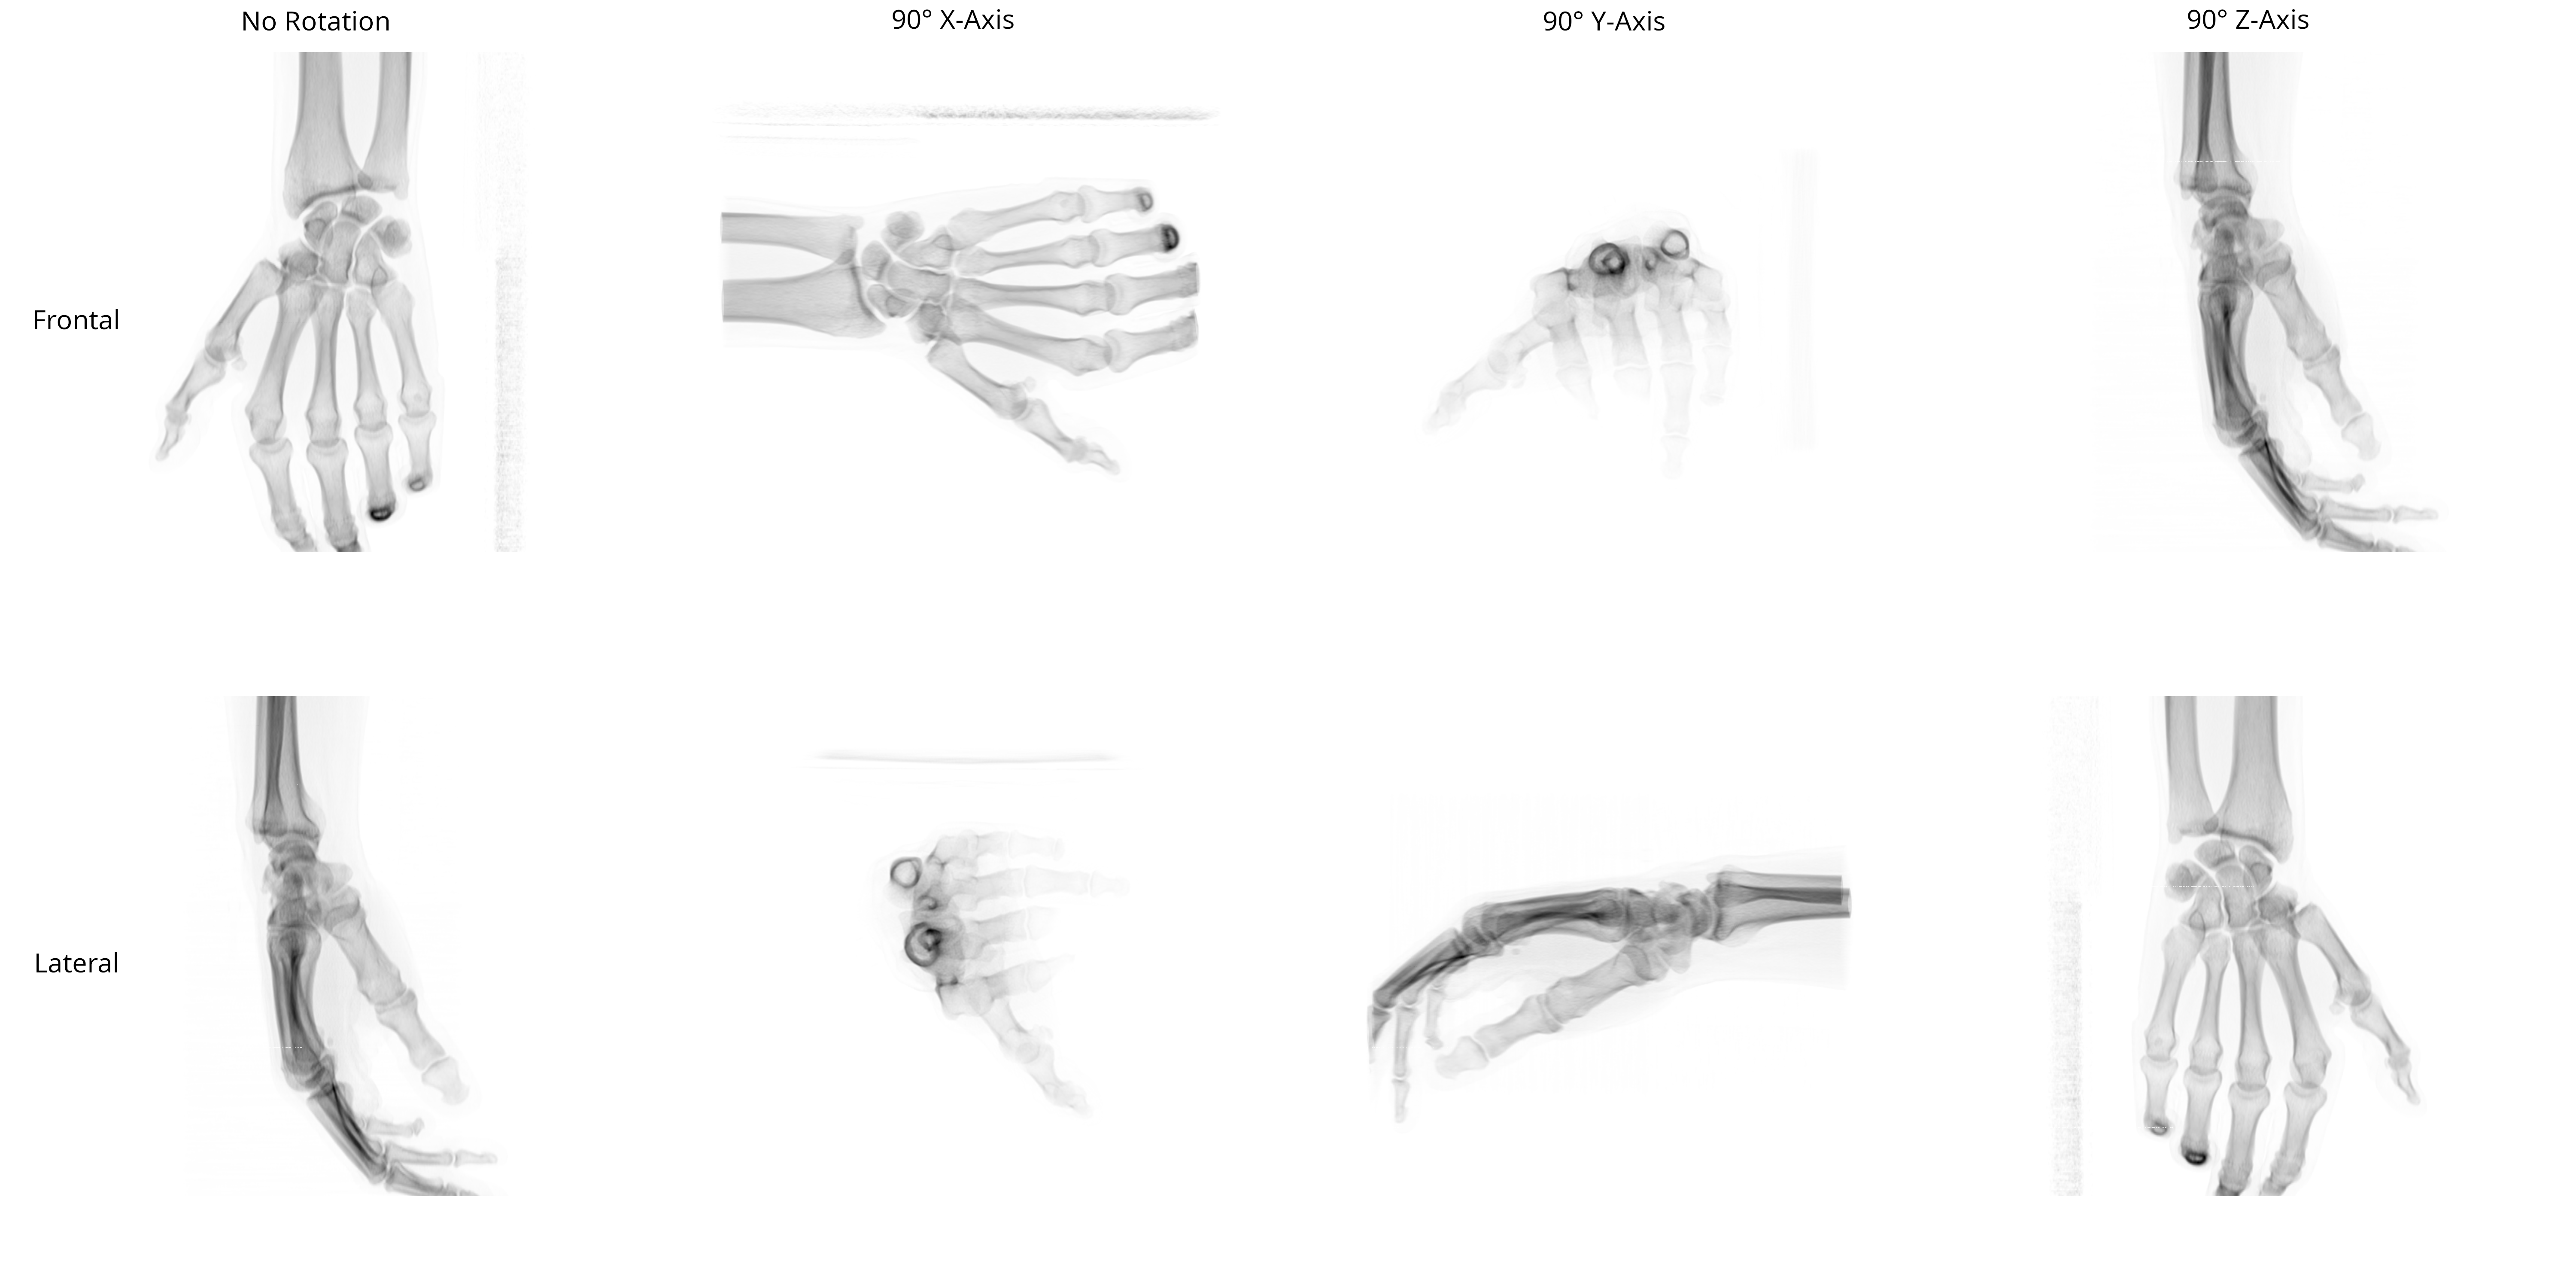
\includegraphics[width=0.5\textwidth]{img/hand_composite_labled.png}
  \end{center}
  \caption{Hand model projections}
\end{figure}

\begin{figure}[H]
  \begin{center}
    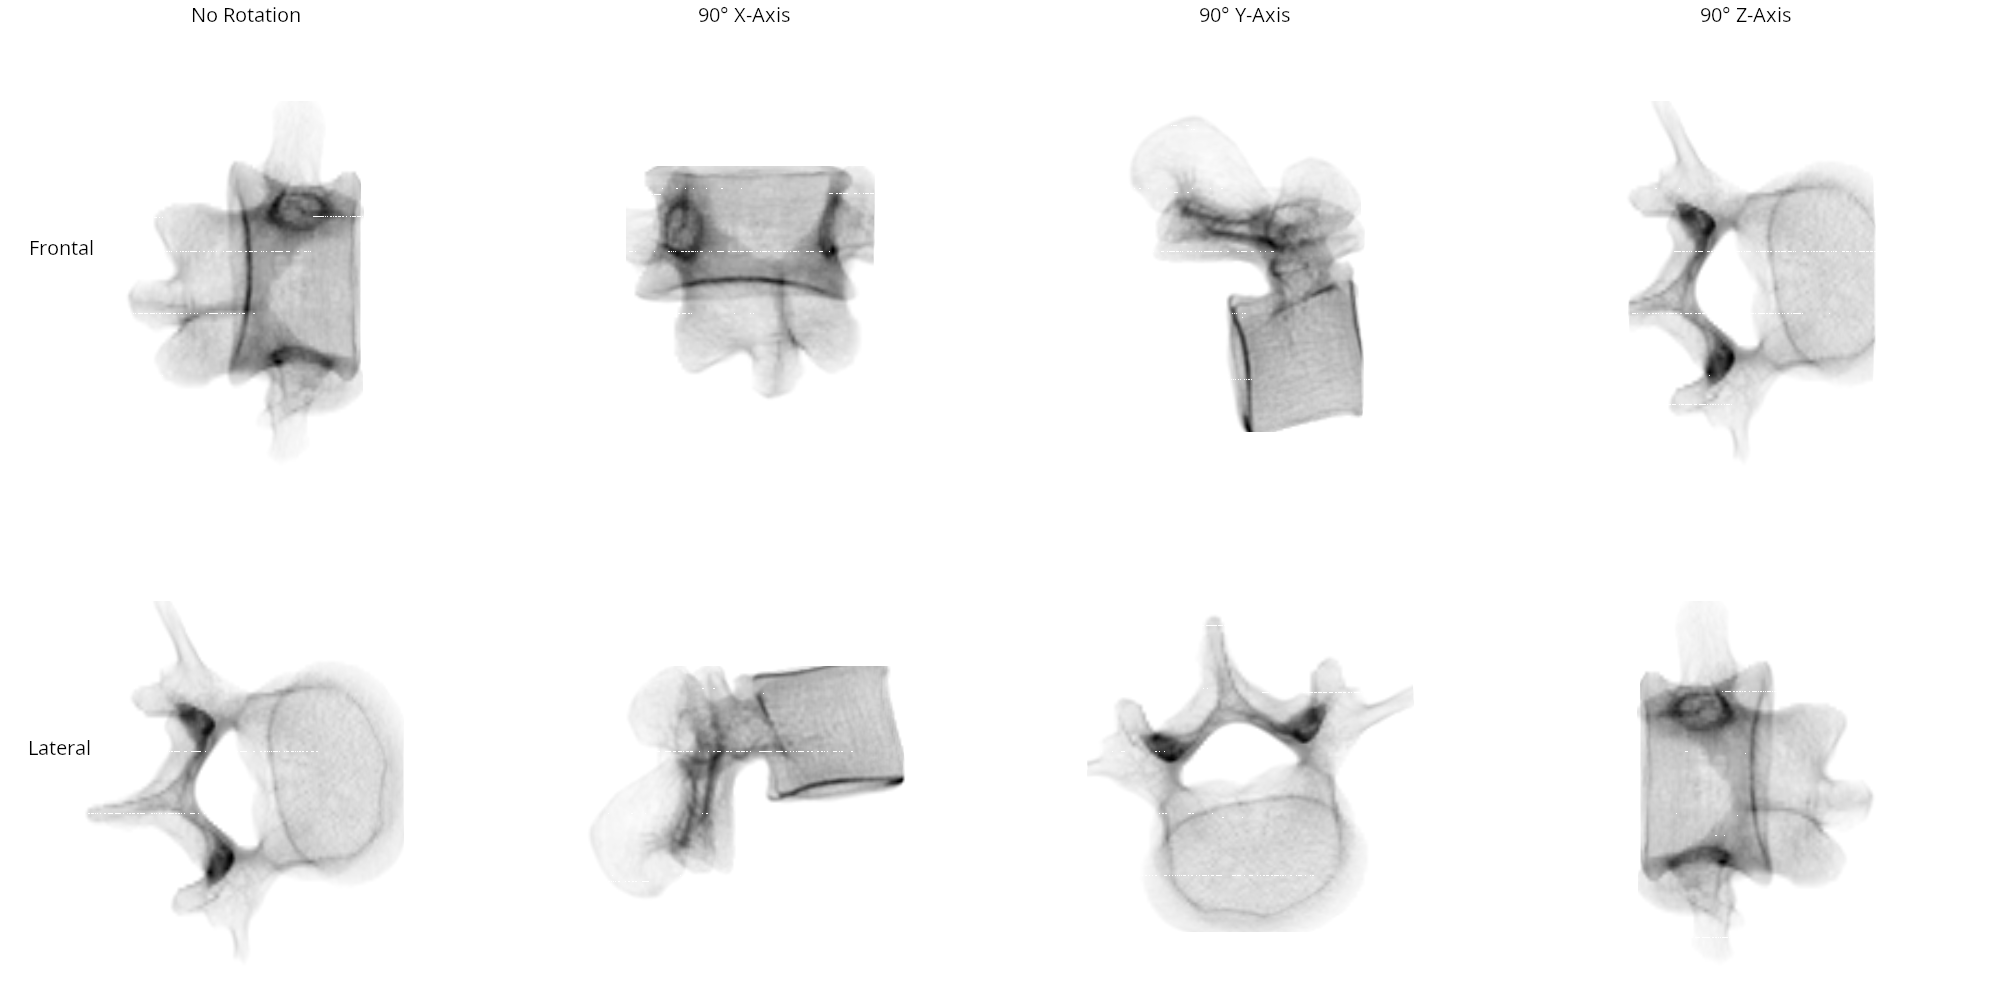
\includegraphics[width=0.5\textwidth]{img/vertabrate-composite_labled.png}
  \end{center}
  \caption{Vertebrate model projections}
\end{figure}


\section{Future work}
Despite the achievements made by this project, there is still a substantial amount of work that can still be done. 
The currently implementation of the geometry utilizes Eigen3 \cite{eigenweb} for all of the linear algebra needs, 
such as matrix and vector multiplication. The primary loop that iterates over each pixel in the final DRR image, is
written in standard C plus plus for the ease of readability and debugging purposes, however, this loop was 
multi threaded using OpenMP \cite{dagum1998openmp} for the interest of performance.
Since, the ultimate goal of this prototype is to end up being integrated into Autoscoper \cite{AKHBARI2019120}, 
2D to 3D registration software, some major refactoring will be needed. Since Autoscoper utilizes a bespoke library
for performing these linear algebra based calculations. Autoscoper is also written in CUDA and OpenCL, so some extra
work would need to be done in order to port the primary loop into a GPU-based kernel.

Additional work should be done to compare the results obtained by this implementation to those generated by 
an EOS\textregistered{} scanner. A possible avenue to perform this comparison would be to position a known volume 
within the physical scanner and collect the radiographs. Then utilizing rotations, position the volume so that appears
in the same location within the DRRs when it is loaded and rendered using this implementation. The two images could 
then be used for template matching. Normalized cross correlation (NCC) \cite{5375779} could be a viable metric to compute the 
similarity between the radiographs and DRRs.

\section{Acknowledgments}

I would like to acknowledge Amy M. Morton and Joseph J. Crisco from Brown University for providing the initial
idea for this project as well as the sample data used in this paper. In addition, I would like to acknowledge 
my project managers Beatriz Paniagua and Jean-Christophe Fillion-Robin for their support and for being indispensable 
technical resources during the course of this project. I would also like to acknowledge my advisers 
Natasha and Sean Banerjee for their support and for proof reading this paper.


\bibliographystyle{plain}

\bibliography{manuscript_references}

\end{document}
